%!TEX root = ../main.tex
\section{Concept \& Design}
\label{sec: concept}
The first part of this section presents the concept, design and the implementation of the MERCURY prototype. The second part describes the Linux kernel modifications that allow Lustre to work with our solution through the posix\_fadvise interface.

The I/O software stack of MERCURY is depicted in Figure~\ref{figure: softwarestack}. Besides the standard I/O libraries we add two software components, an \textit{Assisted I/O library} (AIO), used to intercept I/O calls issued by applications and an \textit{Advice Manager} (AM) process that receives messages sent from the \textit{Assisted I/O library} and generates POSIX advice and GPFS hints. The library is preloaded by the runtime linker before other libraries through the \texttt{LD\_PRELOAD} mechanism and uses UNIX domain sockets to communicate with the \textit{Advice Manager}. In the case of GPFS hints \textit{libgpfs} provides the correct hints API to the \textit{Advice Manager}, other file systems will use the posix\_fadvise syscall.

\begin{figure}[!htb]
  \centering
  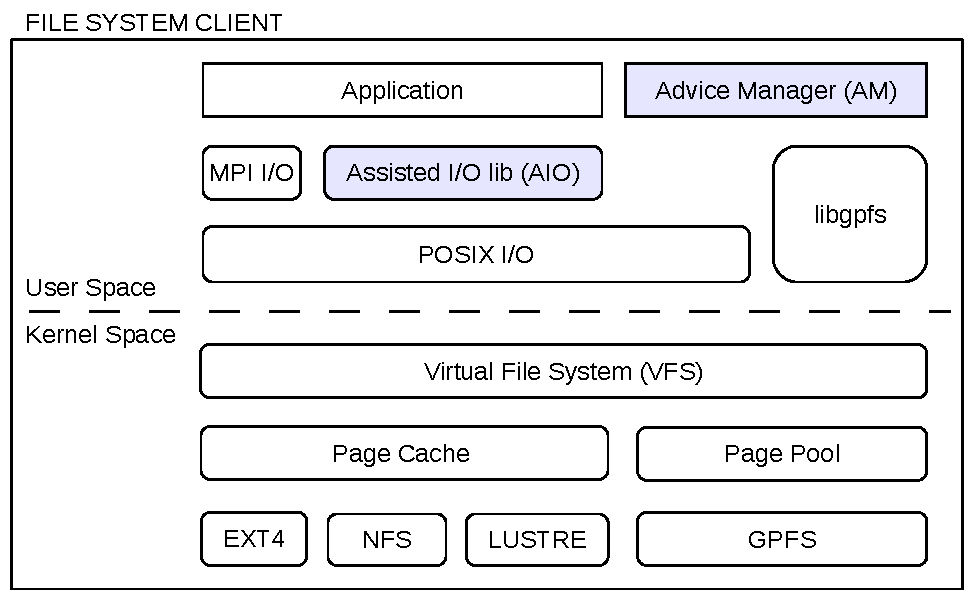
\includegraphics[width=\columnwidth]{figures/softwarestack}
  \caption{MERCURY I/O software stack. \textit{Assisted I/O library} and \textit{Advice Manager} communicate through UNIX domain sockets. %The AM binds its socket to the local file system pathname \texttt{/tmp/channel}, while the IL connects its socket to the same pathname; exactly in the same way they would bind and connect to an IP address if they were located on different nodes in the network. Unix domain sockets are used to pass ancillary data as well as custom messages between the two software entities. 
  Data can reside in a local Linux file system, in Lustre or in GPFS.}
  \label{figure: softwarestack}
\end{figure}

The proposed architecture adds two major contributions. First of all, it allows us to use the Linux advice API as well as the GPFS hints API asynchronously through the \textit{Advice Manager}. This means that we can effectively overlap I/O and computation phases in target applications. Secondly, it enables us to generate POSIX advice and GPFS hints transparently, without the need to modify the application. The information required by the \textit{Advice Manager} is extracted from observations of the application's I/O behaviour~\footnote{How this can be done effectivelly and in a generalized way is itself a research topic and is therefore left as part of future works.} during a set of preliminary runs and then written to a configuration file to be used in following runs.

In the rest of this section we describe the different aspects of our design including the interprocess communication between the two software entities and the prefetching request generation using the \texttt{posix\_fadvise()} system call or the \texttt{gpfs\_fcntl()} function.

\subsection{Interprocess Communication}
\label{subsec: interprocess_comm}
We now describe how interprocess communication is implemented and how messages sent from the \textit{Assisted I/O library} are handled by the \textit{Advice Manager}. Figure~\ref{figure: architecture} depicts the architecture of the two software components introduced by our design. The \textit{Advice Manager} is made up of three smaller modules: a \textit{Request Manager} (RM) that receives requests sent by the \textit{Assisted I/O library}, a \textit{Register Log} (RL) that keeps track of which files are currently handled by the \textit{Advice Manager}, and an \textit{Advisor Thread} (AT) that receives read requests from the \textit{Request Manager} through a queue and issues POSIX advice and GPFS hints.

In order to enable asynchronous prefetching we delegate the task of sending synchronous hints or advice to the \textit{Advice Manager}. When an application issues an open call for a file, the \textit{Assisted I/O library} intercepts it, performs the open and then sends a message to the \textit{Advice Manager}. The message contains a string of the form: \texttt{"\textbf{Register} \textit{pid} \textit{pathname} \textit{fd}"}, plus additional ancillary information explained later. This string tells the \textit{Request Manager} to register the pid of the process opening the file with pathname and file descriptor number, in the register log. As a consequence the \textit{Request Manager} performs two operations, first it asks the \textit{Request Log} to register the new file. From this point on, future read calls for the file will be monitored by the \textit{Advice Manager}. Second, it creates a new \textit{Advisor Thread} that will take care of generating POSIX advice or GPFS hints depending on which file system the file resides in. I/O calls coming from the application are never blocked by the \textit{Assisted I/O library}. The reason is that the \textit{Advice Manager} can become congested by too many requests coming from different processes and we do not want to reflect this on the behaviour of the application.  %The register operation is described by the flow diagram shown in Figure~\ref{figure: register_operation}.

\begin{figure}[!htb]
  \centering
  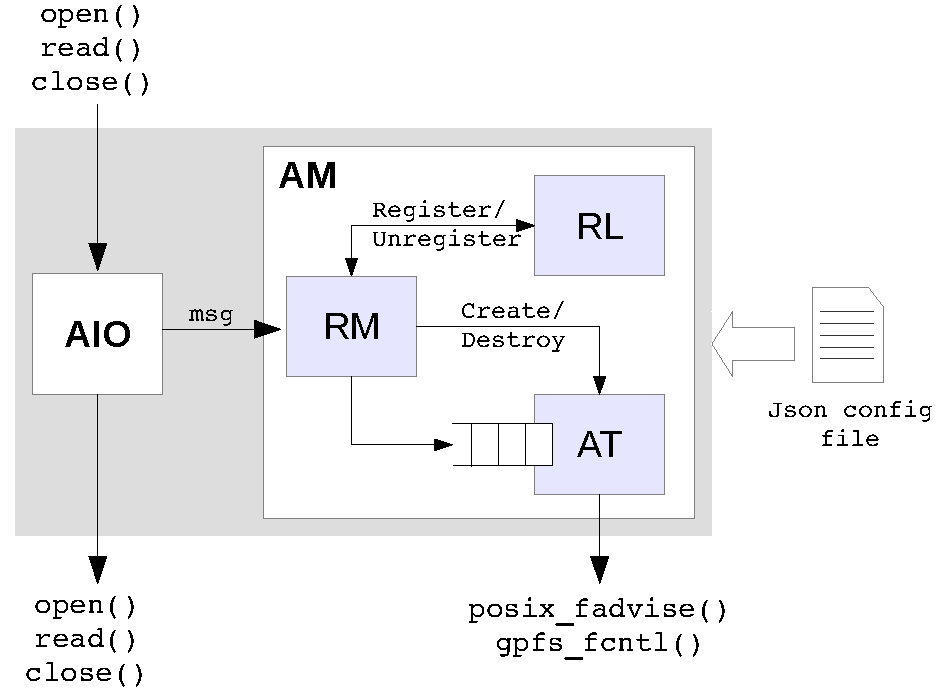
\includegraphics[width=\columnwidth]{figures/architecture}
  \caption{Detailed architecture for the \textit{Advice Manager} (AM) component. This can be further divided into three blocks: \textit{Request Manager} (RM), \textit{Register Log} (RL), and \textit{Advisor Thread} (AT).}
  \label{figure: architecture}
\end{figure}

Both POSIX advice and GPFS hints affect an open file, identified by its file descriptor number. For the \textit{Advice Manager} to send advice or hints on behalf of the application, it needs to share the open file with the application. When sending messages from the \textit{Assisted I/O library} to the \textit{Advice Manager} we use \texttt{sendmsg()}. Besides normal data, this system call allows the transfer of ancillary (or control) information. One use of such information is to send a remote process a 'file descriptor'~\cite{StevensR13} via a UNIX domain socket~\cite{UnixSock}. These numbers are just an index into the kernel's list of a process's open files. When sending a file descriptor using \texttt{sendmsg()}, the kernel copies a new reference to the open file descriptor, and adds it to the receiving process's open files list. The \textit{Advice Manager} receives a new file descriptor number, (which will likely be different to the number sent), which points to a file descriptor shared with the application. This allows us to send hints or advice for the shared file.

\subsection{File Data Prefetching}
\label{subsec: data_prefetching}
POSIX advice and GPFS hints are issued using the \textit{Advisor Thread} created by the \textit{Request Manager} during the register operation (Figure~\ref{figure: architecture}). When an application performs a read operation for an open file, the \textit{Assisted I/O library} sends to the \textit{Advice Manager} a message containing a string of the form: \texttt{"\textbf{Read} \textit{pid} \textit{fd} \textit{off} \textit{len}"}. This string includes the pid of the process, the application's file descriptor number for the file, the offset within the file and the length of the request. The pid and the file descriptor number are used by the \textit{Request Manager} module only to identify the corresponding \textit{Advisor Thread}. When the correct thread has been identified the \textit{Request Manager} pushes the offset and the length of the read request into a queue. This queue is accessed by the \textit{Advisor Thread} that uses the read information to trigger prefetch requests using the local file descriptor and keeps track of all the prefetched data using a block cache data structure. %Figure~\ref{figure: read_operation} shows the flow diagram for the read operation. 

The \textit{Advisor Thread} uses \texttt{posix\_fadvise()} and \texttt{gpfs\_fcntl()} to generate prefetch requests for the underlying file systems (Figure~\ref{figure: architecture}). For files residing in local file systems and Lustre, the \texttt{POSIX\_FADV\_WILLNEED} advice from Table~\ref{table: advice_table} is used to bring the data into the kernel page cache. For files residing in GPFS the \texttt{accRangeArray} in the \texttt{gpfsMultipleAccessRange\_t} data structure in Listing~\ref{mar} is used to define which blocks of the file should be brought into the GPFS internal cache (page pool). 
The size of the file regions to prefetch is defined in a Json\footnote{Open standard format that uses human-readable text to transmit data objects consisting of attribute-value pairs (http://www.rfc-editor.org/rfc/rfc7159.txt).} configuration file, loaded at startup by both the \textit{Advice Manager} and the \textit{Assisted I/O library}. This is the only point of configuration for the user and it contains, besides other information, a list of files and directories that the \textit{Assisted I/O library} should monitor. An example configuration file is shown below. 
\lstset{
        captionpos=b,
        language=python,
        keywordstyle=\color{blue}\footnotesize\ttfamily,
        breaklines=true,
        basicstyle=\footnotesize\ttfamily,
        caption={Example of Json configuration file.},
        label=config
}
\begin{lstlisting}[frame=single]
{
    "File": [
    {
        "Path": "/path/to/target/file",
        "BlockSize": 4194304,
        "CacheSize": 8,
	"ReadAheadSize": 4,
        "WillNeed": [
        {
            "Offset": 0,
            "Length": 0
        }]
    }],
    "Directory": [
    {
        "Path": "/path/to/target/dir",
        "Random": [
        {
            "Offset": 0,
            "Length": 0
        }]
    }]
}
\end{lstlisting}
As it can be seen in Listing~\ref{config} the structure of the configuration file is very simple. It allows users to define which files POSIX advice or GPFS hints should be applied to by setting the `Path' field to the full file path and the regions of the file that are likely to be accessed in terms of offset and length. In the case of POSIX advice users can also define directories to which a global advice should be applied (e.g. randomly accessed files in the directory). Additionally, when indicating a `WillNeed' advice users can directly control the caching behaviour of the \textit{Advisor Thread} block cache. In particular, they can define the granularity of the prefetch request (`BlockSize'), how many blocks can be fitted into the \textit{Advisor Thread} cache (`CacheSize') and how many blocks of data should be read ahead starting from the current accessed block (`ReadAheadSize'). % and in general the configuration file can contain precise information describing the I/O behavior of the application. %In conclusion, by providing configuration files that can match file names, file sizes or even file regions advice and hints should be applied to, administrators or automatized tools can dynamically change the I/O prefetch patterns in order to best fit their needs.
%TODO: is there a citation available for advice on directories?
Clearly the example in Listing~\ref{config} is not exhaustive. More complex configuration files can be generated by administrators (or automatic tools) to dynamically change the I/O patterns of applications in order to best adapt them to the underlying storage system. %For example there may be a preferred block size for files stored in a particular file system

%\begin{algorithm}[h]
% \KwData{sequence of prefetch ranges: \textit{config}, current request offset and length: \{\textit{off}, \textit{len}\}}
% \KwResult{a prefetch request vector: \textit{prefetch}} 
% \While{true}{
%  $off \leftarrow request\ offset$\;
%  $len \leftarrow request\ length$\;
%  \eIf{understand}{
%   go to next section\;
%   current section becomes this one\;
%   }{
%   go back to the beginning of current section\;
%  }
% }
% \caption{GPFS Prefetching Algorithm in the Advisor Thread.}
%\end{algorithm}
The replacement policy for the block cache in the \textit{Advisor Thread} uses an LRU algorithm. In order to prefetch data, the open file is divided into blocks of size `BlockSize' and entire blocks are loaded/released into/from memory as the application progresses. In the case of GPFS the \texttt{accRangeArray} hint is used to prefetch up to `ReadAheadSize' blocks ahead starting from the block touched by the current request. When the number of blocks in the cache has reached `CacheSize', if more blocks are requested, older blocks will be released using the \texttt{relRangeArray} hint to make space for the new ones. In the case of POSIX advice, the behaviour is the same but blocks are loaded into memory using the \texttt{POSIX\_FADV\_WILLNEED} advice and released using the \texttt{POSIX\_FADV\_DONTNEED} advice. The hints interface is automatically selected by the \textit{Advice Manager} at runtime depending on the file system hosting the target file. 
%The only exception is when the prefetch region is bigger than 16MB. In this case the file range is broken down into smaller ranges of 4MB and each of them is prefetched separately. This prevents a very large `WillNeed' section from flooding the page cache at one time (e.g. if the all data of a big file has to be prefetched sequentially). 
%By keeping track of what data has been already prefetched the \textit{Advisor Thread} can also avoid new coming requests triggering the prefetch of the same data. 
%During the time between an open and a close operation the \textit{Advisor Thread} also avoids multiple reads triggering advice and (or) hints for the same block in the file by keeping track of all the currently prefetched blocks. If a new read requests a block already prefetched the read will be ignored. When a block is no longer needed the \textit{Advisor Thread} releases it using either \texttt{POSIX\_FADV\_DONTNEED} or the \texttt{relRangeArray} in Listing~\ref{mar}. 

The \textit{Advisor Thread} block cache also provides a very basic level of coordination among processes accessing the same file. In fact, different \textit{Advisor Thread} instances hinting the same file on behalf of different processes share the same block cache. Blocks requested by one process will appear in the block cache and future accesses to those blocks by other processes will not trigger new prefetching requests.

%At the moment the prefetching algorithm used by the \textit{Advisor Thread} is very simple. It assumes that file ranges in a \texttt{WillNeed} section of the configuration file are accessed in sequential order by the application. In the case of GPFS the \texttt{accRangeArray} is used to prefetch up to \texttt{GPFS\_MAX\_RANGE\_COUNT} blocks ahead of the current request. When the application requests data that is \texttt{GPFS\_MAX\_RANGE\_COUNT/2} blocks away from the last prefetched block, another eight blocks of data are prefetched. On the other hand requested blocks that are no longer needed are released in groups of \texttt{GPFS\_MAX\_RANGE\_COUNT/2} using the \texttt{relRangeArray}. In the case of POSIX advice the algorithm is the same but instead of blocks it considers file ranges contained in the \texttt{WillNeed} section as a single prefetch unit for \texttt{POSIX\_FADV\_WILLNEED}. By keeping track of what data in the file has been already prefetched the \textit{Advisor Thread} can prevent new requests from triggering a prefetch of the same data. %During the time between an open and a close operation the \textit{Advisor Thread} also avoids multiple reads triggering advice and (or) hints for the same block in the file by keeping track of all the currently prefetched blocks. If a new read requests a block already prefetched the read will be ignored. When a block is no longer needed the \textit{Advisor Thread} releases it using either \texttt{POSIX\_FADV\_DONTNEED} or the \texttt{relRangeArray} in Listing~\ref{mar}. 
%\todo[inline]{this should be replaced or extended by a formal description of the algorithm ...}

In general the configuration file can be used to describe any of the advice listed in Table~\ref{table: advice_table} and the hints listed in Table~\ref{table: hints_table}. To define a new scenario, we may consider a file region accessed sequentially for which the \texttt{POSIX\_FADV\_SEQUENTIAL} advice type could be used, and another region accessed randomly for which the \texttt{POSIX\_FADV\_RANDOM} advice type could be used. In this case, the configuration file would contain a list of file regions, specifying which type of advice messages are suitable. The right advice will be selected according to which part of the file is being accessed currently. This feature allows us to overcome another limitation of the Linux advice implementation that has been mentioned in Section~\ref{subsec: posix_advice_api}, namely, the first three advice types apply to the whole file since the implementation in the kernel completely disregards the byte ranges specified by the user.
 
Finally, when the application closes the file the \textit{Assisted I/O library} sends to the \textit{Advice Manager} a message containing a string of the form: \texttt{"\textbf{Unregister} \textit{pid} \textit{fd}"}. This string includes the pid of the process and the file descriptor number of the file to be closed. In response to this request the \textit{Request Manager} tells the \textit{Register Log} to unregister the file and destroys the \textit{Advisor Thread}, it also closes its shared copy of the file.

\subsection{POSIX Advice integration with Lustre}
\label{subsec: posix_advice_lustre}
Lustre is a high performance parallel file system for Linux clusters. It works in kernel space and takes advantage of the available page cache infrastructure. Additionally, it extends POSIX read and write operations with distributed locks to provide data consistency across the whole cluster. Even though Lustre makes use of the Linux kernel page cache, the previously described POSIX advice syscall has no effect on Lustre. The reason can be understood by looking at Figure~\ref{figure: kernel}. This reports the simplified call graph for the Lustre read operation in the file system client. To simplify the explanation, the figure is divided into four quadrants. Along the x-axis we have the native kernel functions (e.g. \texttt{generic\_file\_aio\_read}), separated by the Lustre specific functions (e.g. \texttt{lustre\_generic\_file\_read}). Along the y-axis we have page operations (e.g. \texttt{find\_get\_page}) separated by the file operations (e.g. \texttt{generic\_file\_aio\_read}). 

We can notice that Lustre extends the kernel code with additional file and page operations through the Lustre Lite component. These are the functions used by the kernel to fill the file operations table and the address space operations table. The \texttt{posix\_fadvise()} system call in the kernel translates into \texttt{fadvise64()}. In the case of \texttt{POSIX\_FADV\_WILLNEED} this function directly invokes \texttt{force\_page\_cache\_readahead()} which has no effect on \texttt{ll\_readpage()}. Other advice such as \texttt{POSIX\_FADV\_\{NORMAL,SEQUENTIAL,RANDOM\}} are disabled in Lustre by setting the kernel read-ahead window size to zero. This is done so that lustre will not speculatively try to gain a highly-contended lock to fulfil an optimistic read-ahead request.

\begin{figure}[!htb]
  \centering
  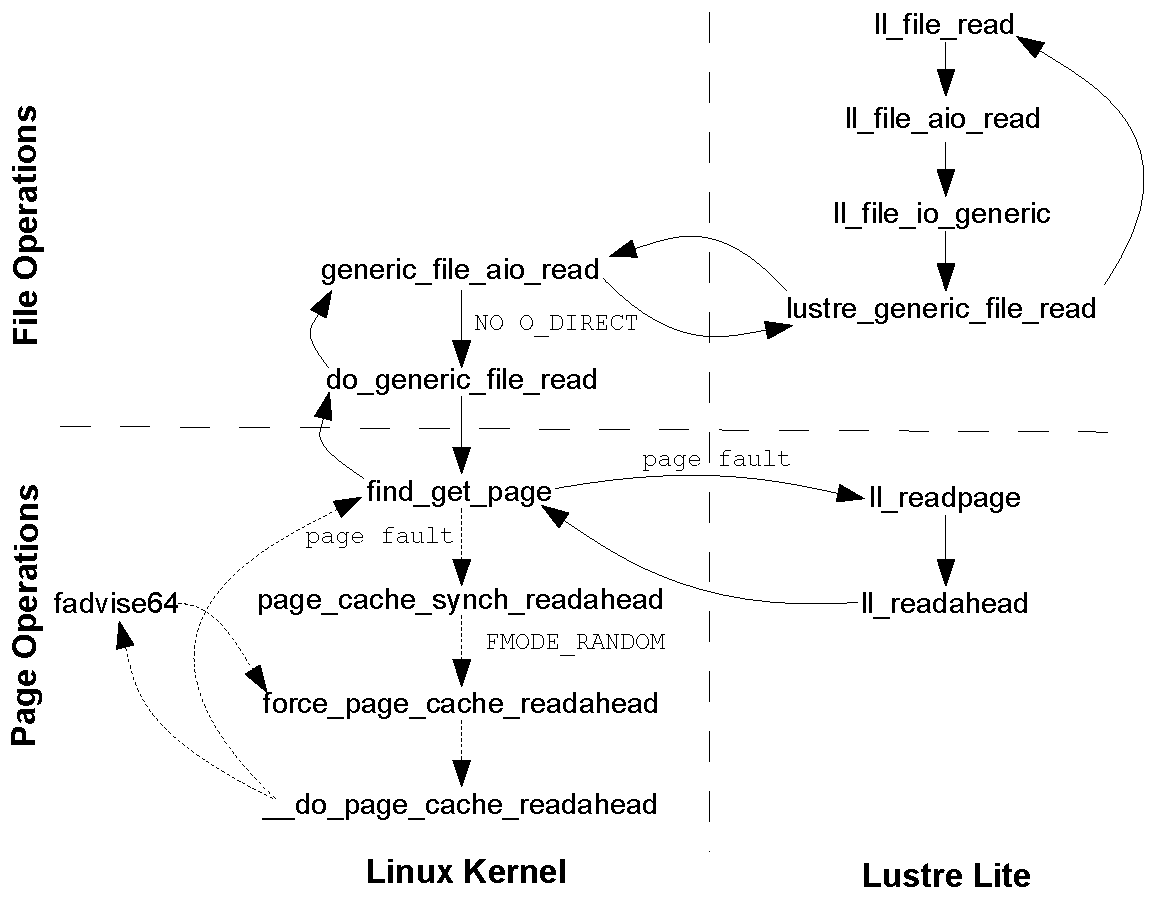
\includegraphics[width=\columnwidth]{figures/kernel}
  \caption{Simplified function call graph for the read operation in Lustre. For page operations in the Linux kernel the picture also shows the call graph typically followed by local reads as well as the call graph for the \texttt{POSIX\_FADV\_WILLNEED} advice in the \texttt{posix\_fadvise()} implementation (dashed line).}
  \label{figure: kernel}
\end{figure}

% This paragraph could be explained more clearly - you are effectivly filling the file system cache, on the assumption that it is the page-cache, instead of filling the page cache. This allows file systems that don't interface directly with the page cache to work.
In order to enable \texttt{POSIX\_FADV\_WILLNEED} in Lustre we modified the call graph of \texttt{fadvise64()} presented in Figure~\ref{figure: kernel} to invoke the \texttt{aio\_read()} operation in the file operations table for the open file and block until all the data has been read into the page cache. In this way we can force the kernel to invoke the corresponding file read operation in Lustre, acquiring locks as appropriate. Of course this mechanism still works with local file systems which eventually will end up calling \texttt{force\_page\_cache\_readahead()} as in the original version.

To prevent the new generated read from altering the read-ahead state of normal read operations, in \texttt{fadvise64()} we create a new \texttt{struct file} using the \texttt{dentry\_open()} routine and set the access mode flag (\texttt{f\_mode}) of the new file to \texttt{FMODE\_RANDOM} (which is exactly what the \texttt{POSIX\_FADV\_RANDOM} advice message does to disable read-ahead for random accessed files). This mechanism works perfectly with local file systems but has no effect on Lustre's read-ahead algorithm which is independent from the Linux kernel read-ahead. Therefore, \texttt{POSIX\_FADV\_WILLNEED} in the case of Lustre prefetches a bit more data than requested. This is acceptable for now but a future implementation will also modify the Lustre code to make sure the behaviour is the same in both cases.

Finally, our kernel patch does not require any user buffer to be provided with the new read operation. To avoid data being copied to user space we pass a null pointer to the \texttt{aio\_read()} routine. Additionally we defined a new \texttt{ki\_flag} for the kernel I/O control block (\texttt{kiocb}), that we called \texttt{KIF\_FORCE\_READ\_AHEAD}. This new flag is checked in the \texttt{generic\_file\_aio\_read()} routine and if set the \texttt{do\_generic\_file\_read()} routine is invoked with a pointer to the \texttt{file\_read\_actor\_dummy()} routine. \texttt{file\_read\_actor()} is normally the routine responsible for copying the data from the page cache to the user space buffer. Since in our case there is no user space buffer, the dummy routine just returns success.
